%!TEX program = xelatex
% 完整编译: xelatex -> biber/bibtex -> xelatex -> xelatex
\documentclass[lang=cn,a4paper,newtx]{elegantpaper}

\title{ElegantPaper: 一个优美的 \LaTeX{} 工作论文模板}
\author{作者1 \\ 某某大学/机构 \and 作者2 \\ 某某大学/机构}
\institute{\href{https://elegantlatex.org/}{Elegant\LaTeX{} 项目组}}

\version{0.11}
\date{\zhdate{2022/12/31}}

% 本文档命令
\usepackage{array}
\newcommand{\ccr}[1]{\makecell{{\color{#1}\rule{1cm}{1cm}}}}
\addbibresource[location=local]{reference.bib} % 参考文献,不要删除

\begin{document}

\maketitle

\begin{abstract}
本文为 \href{https://github.com/ElegantLaTeX/ElegantPaper/}{ElegantPaper} 的说明文档。此模板基于 \LaTeX{} 的 article 类,专为工作论文写作而设计。设计这个模板的初衷是让作者不用关心工作论文的格式,专心写作,从而有更加舒心的写作体验。如果你有其他问题、建议或者报告 bug,可以在 \href{https://github.com/ElegantLaTeX/ElegantPaper/issues}{GitHub::ElegantPaper/issues} 留言。如果你想了解更多 Elegant\LaTeX{} 项目组设计的模板,请访问 \href{https://github.com/ElegantLaTeX/}{GitHub::ElegantLaTeX}。
\keywords{Elegant\LaTeX{},工作论文,模板}
\end{abstract}

\section{模板使用须知}

\textcolor{red}{\bfseries 本模板自 2023 年 1 月 1 日开始,不再维护,不建议使用本系列模板!为了保证之前版本的用户仍然能查到说明文档,本说明文档仍然保留过去的信息。}

\subsection{注意事项}
\textbf{文献部分}:我们将 bibtex 的默认文献编译方式改为 biblatex,不过我们也提供了两个后端,\lstinline{bibend=biber} 和 \lstinline{bibend=bibtex}。特别需要注意的是从 0.10 开始,文献文件改为 \lstinline{reference.bib},与 ElegantBook 保持一致,而参考文献的引文样式等更多格式,请参考后文参考文献部分,更多样式可以参考 biblatex 文档。 

\textbf{字体部分},我们将 newtxtext 宏包的支持方式改为了字体名称设定方式,设定英文字体为 TeX Gyre Terms/Heros,英文字体部分,根据编译方式选择不同字体。对于一般用户而言,不太需要关心这部分内容。

另外,中文请务必使用 \hologo{XeLaTeX} 编译。

\subsection{模板介绍}

此模板基于 \LaTeX{} 的标准文类 article 设计,所以 article 文类的选项也能传递给本模板,比如 \lstinline{a4paper, 11pt} 等等。

\begin{lstlisting}
\documentclass[a4paper,11pt]{elegantpaper}
\end{lstlisting}

\textbf{注意}:Elegant\LaTeX{} 系列模板已经全部上传至 \href{https://www.overleaf.com/latex/templates/elegantpaper-template/yzghrqjhmmmr}{Overleaf} 上,用户可以在线使用。另外,为了方便国内用户,模板也已经传至\href{https://gitee.com/ElegantLaTeX/ElegantPaper}{码云}。


\subsection{全局选项}
此模板定义了一个语言选项 \lstinline{lang},可以选择英文模式 \lstinline{lang=en}(默认)或者中文模式 \lstinline{lang=cn}。当选择中文模式时,图表的标题引导词以及参考文献,定理引导词等信息会变成中文。你可以通过下面两种方式来选择语言模式:
\begin{lstlisting}
\documentclass[lang=cn]{elegantpaper} % or
\documentclass[cn]{elegantpaper} 
\end{lstlisting}

\textbf{注意:} 英文模式下,由于没有添加中文宏包,无法输入中文。如果需要输入中文,可以通过在导言区引入中文宏包 \lstinline{ctex} 或者加入 \lstinline{xeCJK} 宏包后自行设置字体。 
\begin{lstlisting}
\usepackage[UTF8,scheme=plain]{ctex}
\end{lstlisting}

\subsection{数学字体选项}

本模板定义了一个数学字体选项(\lstinline{math}),可选项有三个:
\begin{enumerate}
  \item \lstinline{math=cm}(默认),使用 \LaTeX{} 默认数学字体(推荐,无需声明);
  \item \lstinline{math=newtx},使用 \lstinline{newtxmath} 设置数学字体(潜在问题比较多)。
  \item \lstinline{math=mtpro2},使用 \lstinline{mtpro2} 宏包设置数学字体,要求用户已经成功安装此宏包。
\end{enumerate}

\subsection{中文字体选项}

模板提供中文字体选项 \lstinline{chinesefont},可选项有
\begin{enumerate}
  \item \lstinline{ctexfont}:默认选项,使用 \lstinline{ctex} 宏包根据系统自行选择字体,可能存在字体缺失的问题,更多内容参考 \lstinline{ctex} 宏包\href{https://ctan.org/pkg/ctex}{官方文档}\footnote{可以使用命令提示符,输入 \lstinline{texdoc ctex} 调出本地 \lstinline{ctex} 宏包文档}。
  \item \lstinline{founder}:方正字体选项(\textbf{需要安装方正字体}),后台调用 \lstinline{ctex} 宏包并且使用 \lstinline{fontset=none} 选项,然后设置字体为方正四款免费字体,方正字体下载注意事项见后文,用户只需要安装方正字体即可使用该选项。
  \item \lstinline{nofont}:后台会调用 \lstinline{ctex} 宏包并且使用 \lstinline{fontset=none} 选项,不设定中文字体,用户可以自行设置中文字体,具体见后文。
\end{enumerate}

\subsubsection{方正字体选项}
由于使用 \lstinline{ctex} 宏包默认调用系统已有的字体,部分系统字体缺失严重,因此,用户希望能够使用其它字体,我们推荐使用方正字体。方正的{\songti 方正书宋}、{\heiti 方正黑体}、{\kaishu 方正楷体}、{\fangsong 方正仿宋}四款字体均可免费试用,且可用于商业用途。用户可以自行从\href{http://www.foundertype.com/}{方正字体官网}下载此四款字体,在下载的时候请\textbf{务必}注意选择 GBK 字符集,也可以使用 \href{https://www.latexstudio.net/}{\LaTeX{} 工作室}提供的\href{https://pan.baidu.com/s/1BgbQM7LoinY7m8yeP25Y7Q}{方正字体,提取码为:njy9} 进行安装。安装时,{\kaishu Win 10 用户请右键选择为全部用户安装,否则会找不到字体。}

\begin{figure}[!htb]
\centering
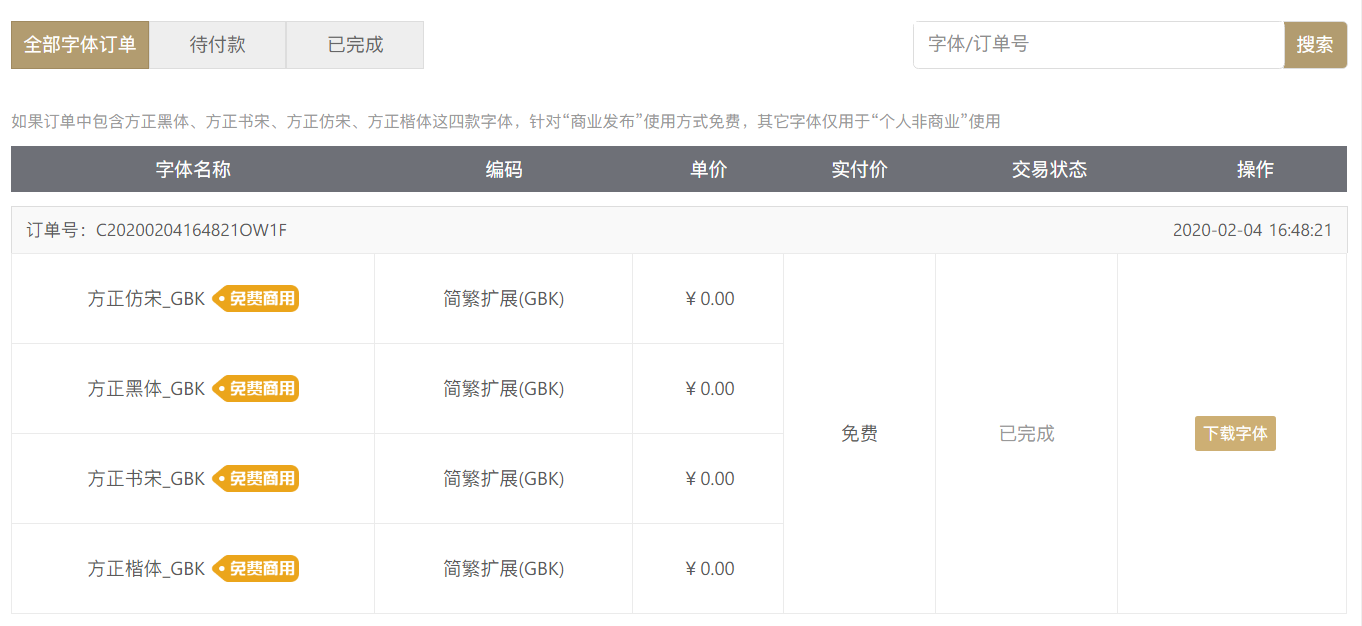
\includegraphics[width=0.9\textwidth]{founder.png}
\end{figure}

\subsubsection{其他中文字体}
如果你想完全自定义字体\footnote{这里仍然以方正字体为例。},你可以选择 \lstinline{chinesefont=nofont},然后在导言区设置即可,可以参考下方代码:
\begin{lstlisting}
\setCJKmainfont[BoldFont={FZHei-B01},ItalicFont={FZKai-Z03}]{FZShuSong-Z01}
\setCJKsansfont[BoldFont={FZHei-B01}]{FZKai-Z03}
\setCJKmonofont[BoldFont={FZHei-B01}]{FZFangSong-Z02}
\setCJKfamilyfont{zhsong}{FZShuSong-Z01}
\setCJKfamilyfont{zhhei}{FZHei-B01}
\setCJKfamilyfont{zhkai}[BoldFont={FZHei-B01}]{FZKai-Z03}
\setCJKfamilyfont{zhfs}[BoldFont={FZHei-B01}]{FZFangSong-Z02}
\newcommand*{\songti}{\CJKfamily{zhsong}}
\newcommand*{\heiti}{\CJKfamily{zhhei}}
\newcommand*{\kaishu}{\CJKfamily{zhkai}}
\newcommand*{\fangsong}{\CJKfamily{zhfs}}
\end{lstlisting}



\subsection{自定义命令}
此模板并没有修改任何默认的 \LaTeX{} 命令或者环境\footnote{目的是保证代码的可复用性,请用户关注内容,不要太在意格式,这才是本工作论文模板的意义。}。另外,本模板可以使用的 4 个额外命令:
\begin{enumerate}
  \item \lstinline{\email}:创建邮箱地址的链接,比如 \email{xxx@outlook.com};
  \item \lstinline{\figref}:用法和 \lstinline{\ref} 类似,但是会在插图的标题前添加 <\textbf{图 n}> ;
  \item \lstinline{\tabref}:用法和 \lstinline{\ref} 类似,但是会在表格的标题前添加 <\textbf{表 n}>;
  \item \lstinline{\keywords}:为摘要环境添加关键词。
\end{enumerate}

\subsection{参考文献}

文献部分,本模板调用了 biblatex 宏包,并提供了 biber(默认) 和 bibtex 两个后端选项,可以使用 \lstinline{bibend} 进行修改:

\begin{lstlisting}
  \documentclass[bibtex]{elegantpaper}
  \documentclass[bibend=bibtex]{elegantpaper}
\end{lstlisting}

关于文献条目(bib item),你可以在谷歌学术,Mendeley,Endnote 中取,然后把它们添加到 \lstinline{reference.bib} 中。在文中引用的时候,引用它们的键值(bib key)即可。

为了方便文献样式修改,模板引入了 \lstinline{bibstyle} 和 \lstinline{citestyle} 选项,默认均为数字格式(numeric),参考文献示例:\cite{cn1,en2,en3} 使用了中国一个大型的 P2P 平台(人人贷)的数据来检验男性投资者和女性投资者在投资表现上是否有显著差异。

如果需要设置为国标 GB7714-2015,需要使用:
\begin{lstlisting}
  \documentclass[citestyle=gb7714-2015, bibstyle=gb7714-2015]{elegantpaper} 
\end{lstlisting}

如果需要添加排序方式,可以在导言区加入
\begin{lstlisting}
  \ExecuteBibliographyOptions{sorting=ynt}
\end{lstlisting}

启用国标之后,可以加入 \lstinline{sorting=gb7714-2015}。


\section{使用 newtx 系列字体}

如果需要使用原先版本的 \lstinline{newtx} 系列字体,可以通过显示声明数学字体:

\begin{lstlisting}
\documentclass[math=newtx]{elegantpaper}
\end{lstlisting}

\subsection{连字符}

如果使用 \lstinline{newtx} 系列字体宏包,需要注意下连字符的问题。
\begin{equation}
  \int_{R^q} f(x,y) dy.\emph{of\kern0pt f}
\end{equation}

\begin{lstlisting}
\begin{equation}
  \int_{R^q} f(x,y) dy.\emph{of \kern0pt f}
\end{equation}
\end{lstlisting}

\subsection{宏包冲突}

有用户反馈模板在使用 \lstinline{yhmath} 以及 \lstinline{esvect} 等宏包时会报错:
\begin{lstlisting}
LaTeX Error:
   Too many symbol fonts declared.
\end{lstlisting}

原因是在使用 \lstinline{newtxmath} 宏包时,重新定义了数学字体用于大型操作符,达到了 {\heiti 最多 16 个数学字体} 的上限,在调用其他宏包的时候,无法新增数学字体。为了减少调用非常用宏包,在此给出如何调用 \lstinline{yhmath} 以及 \lstinline{esvect} 宏包的方法。

请在 \lstinline{elegantpaper.cls} 内搜索 \lstinline{yhmath} 或者 \lstinline{esvect},将你所需要的宏包加载语句\textit{取消注释}即可。


\section{常见问题 FAQ}

\begin{enumerate}[label=\arabic*).]
  \item \textit{如何删除版本信息?}\\
    导言区不写 \lstinline|\version{x.xx}| 即可。
  \item \textit{如何删除日期?}\\
    需要注意的是,与版本 \lstinline{\version} 不同的是,导言区不写或注释 \lstinline{\date} 的话,仍然会打印出当日日期,原因是 \lstinline{\date} 有默认参数。如果不需要日期的话,日期可以留空即可,也即 \lstinline|\date{}|。
  \item \textit{如何获得中文日期?}\\
    为了获得中文日期,必须在中文模式下\footnote{英文模式下,由于未加载中文宏包,无法输入中文。},使用 \lstinline|\date{\zhdate{2019/10/11}}|,如果需要当天的汉化日期,可以使用 \lstinline|\date{\zhtoday}|,这两个命令都来源于 \href{https://ctan.org/pkg/zhnumber}{\lstinline{zhnumber}} 宏包。
  \item \textit{如何添加多个作者?}\\
    在 \lstinline{\author} 里面使用 \lstinline{\and},作者单位可以用 \lstinline{\\} 换行。
    \begin{lstlisting}
    \author{author 1\\ org. 1 \and author 2 \\ org. 2 }
    \end{lstlisting}
  \item \textit{如何添加中英文摘要?}\\
    请参考 \href{https://github.com/ElegantLaTeX/ElegantPaper/issues/5}{GitHub::ElegantPaper/issues/5}
\end{enumerate}


\section{致谢}

特别感谢 \href{https://github.com/sikouhjw}{sikouhjw} 和 \href{https://github.com/syvshc}{syvshc}  长期以来对于 Github 上 issue 的快速回应,以及各个社区论坛对于 ElegantLaTeX 相关问题的回复。特别感谢 ChinaTeX 以及 \href{http://www.latexstudio.net/}{LaTeX 工作室} 对于本系列模板的大力宣传与推广。

如果你喜欢我们的模板,你可以在 Github 上收藏我们的模板。

\nocite{*}
\printbibliography[heading=bibintoc, title=\ebibname]

\appendix
%\appendixpage
\addappheadtotoc

\end{document}
